\documentclass{article}
\usepackage[utf8]{inputenc}
\usepackage{listings}
\usepackage{float}
\usepackage{graphicx}

\usepackage{color}
 
\definecolor{codegreen}{rgb}{0,0.6,0}
\definecolor{codegray}{rgb}{0.5,0.5,0.5}
\definecolor{codepurple}{rgb}{0.58,0,0.82}
\definecolor{backcolour}{rgb}{0.95,0.95,0.92}
 
\lstdefinestyle{mystyle}{
    backgroundcolor=\color{backcolour},   
    commentstyle=\color{codegreen},
    keywordstyle=\color{magenta},
    numberstyle=\tiny\color{codegray},
    stringstyle=\color{codepurple},
    basicstyle=\footnotesize,
    breakatwhitespace=false,         
    breaklines=true,                 
    captionpos=b,                    
    keepspaces=true,                 
    numbers=left,                    
    numbersep=5pt,                  
    showspaces=false,                
    showstringspaces=false,
    showtabs=false,                  
    tabsize=2,
    language=python
}
\lstset{style=mystyle}


\title{Tugas Kecerdasan Buatan Section 1}
\author{Ahmad Agung Tawakkal\\
        1184015\\
        D4 TI 3 B}
\date{Maret 2021}

\graphicspath{{figure/}}

\begin{document}

\maketitle

\newpage


\section{Chapter 1}
    \subsection{Teori}
        \begin{enumerate}
            \item Definisi, Sejarah, dan Perkembangan Kecerdasan Buatan
                \begin{itemize}
                    \item Definisi
                        \paragraph{}Kecerdasan Buatan merupakan sebuah sistem yang sangat cerdas, dimana sistem ini dapat digunakan pada sebuah teknologi, misalnya robot yang dapat diajak ngobrol atau robot yang bisa menyelesaikan rubik dengan cepat. Sistem ini memeiliki proses berfikir layaknya manusia.
                    \item Sejarah dan Perkembangan
                        \paragraph{}Riset Kecerdasan Buatan awalnya dikakukan pada tahun 1950, namun Kecerdasan Buatan pertama kali dibuat pada tahun 1956. Kecerdasan Buatan bertujuan untuk membangun sebuah komputer yang memiliki penalaran bagaikan manusia. Pada tahun 1960 Amerika ingin mengembangakan dan melatih komputer agar dapat memiliki penalaran bagaikan manusia. Kemudian pada tahun 1970 Proyek DARPA berhasil menyelesaikan pemetaan jalan, pada tahun 2003 DARPA berhasil menghasilkan asisten pribadi yang cerdas. John McCarthy merupakan bapak AI mendirikan sebuah lembaga AI (Starford Artificial Intelligence Laboratory dan MIT Artificial Intelligence Laboratory). Dilembaga inilah pengembagan inovasi pada bidang AI semakin pesat juga pada lembaga ini memiliki bidang Human Skill, Vision, Listening, Reasoning, dan Moment of Limbs.
                \end{itemize}
                
            \item Definisi Supervised Learning, Klasifikasi, Regresi dan Unsupervised learning. Data set, Training set dan Testing set
                \begin{itemize}
                    \item Supervised Learning
                        \paragraph{}Superviser Learning mempunyai sebuah variable inputan dan varaible ouput serta menggunakan satu algoritma atau banyak untuk memahami fungsi pemetaan dari inputan ke output. Superviser Learning bertujuan untuk memperkirakan fungsi pemetaan, saat kita memiliki sebuah inputan kita dapat memprediksi hasil output dari inputan tersebut.
                    \item Unsuperviser Learning
                        \paragraph{}Unsuperviser Learning mempunyai sebuah variable inputan namun tidak memiliki variable output. Unsuperviser Learning berfungsi untuk memodelkan struktur dasar agar dapat mempelajari data lebih jauh atau meyimpulkan fungsi, mendeskripsikan atau menjelaskan data.
                    \item Klasifikasi
                        \paragraph{}Klasifikasi atau peggolongan daoat menebak suatu kelas tertentu dari sebuah kumpulan data (data set). Pada sekumpulan data ini bisanya memiliki sebuah atribut yang menjadi tujuan klasifikasi. Atribut ini merupakan kolom dari tabel, kemudian diklasifikasi serta juga membutuhkan atribut pendukung agar atribut dapat berpengaruh signifikan terhadap atribut tujuan.
                    \item Regresi
                        \paragraph{}Regresi hampir sama dengan klasifikasi namun yang membedakan adalah regresi memberikan hasil yang tidak terbatas sedangkan klasifikasi memberikan hasil yang terbatas.
                \end{itemize}
        \end{enumerate}
        
    \subsection{Instalasi}
        \begin{enumerate}
            \item Instalasi library scikit dari anaconda
                \paragraph{}Membuka anaconda prompt kemudian masukan perintah berikut \textit{pip install -U scikit-learn}.
                \begin{figure}[ht]
                    \centerline{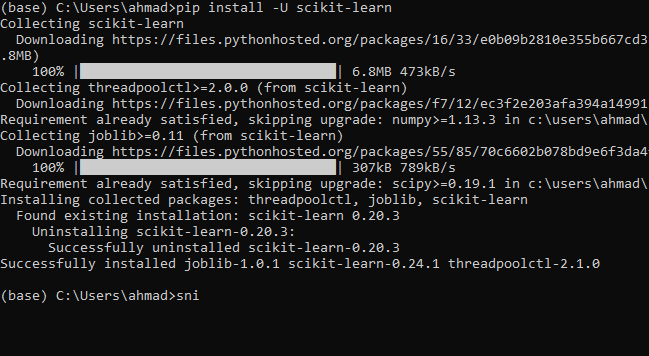
\includegraphics[width=10cm]{1.PNG}}
                \end{figure}
            \newpage
            \item Loading an example dataset
                \begin{figure}[ht]
                    \centerline{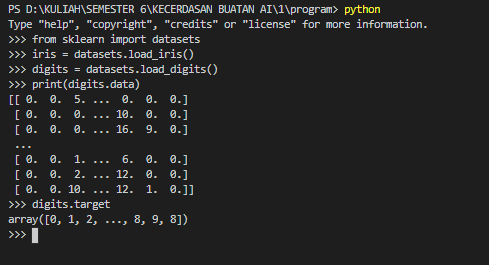
\includegraphics[width=10cm]{2.PNG}}
                \end{figure}
                \begin{itemize}
                    \item from sklearn import datasets
                        \paragraph{}Mengimport datasets dari library sklearn
                    \item iris = datasets.load\_iris()
                        \paragraph{} Membuat sebuah variable iris dengan mengisi fungsi load\_iris() dari file datasets yang telah di import
                    \item digits = datasets.load\_digits()
                        \paragraph{}Membuat sebuah variable digits dengan mengisi fungsi load\_digits() dari file datasets yang telah di import
                    \item print(digits.data)
                        \paragraph{}Menampilkan isi dari variable digits
                    \item digits.target
                        \paragraph{}Menampilkan array angka yang sesuai dengan setiap gambar digit 
                \end{itemize}
                \newpage
            \item Learning and predicting
                \begin{figure}[ht]
                    \centerline{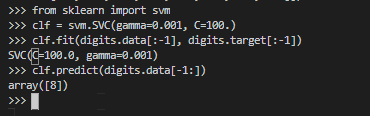
\includegraphics[width=10cm]{3.PNG}}
                \end{figure}
                \begin{itemize}
                    \item from sklearn import svm
                        \paragraph{}Mengimport svm dari library sklearn
                    \item clf = svm.SVC(gamma=0.001, C=100.)
                        \paragraph{}Membuat variable dengan nama clf, dan valuenya dari fungsi SVC yang telah kita import (svm)
                    \item clf.fit(digits.data[:-1], digits.target[:-1])
                    \item clf.predict(digits.data[-1:])
                \end{itemize}
            \item Model persistence
                \begin{figure}[ht]
                    \centerline{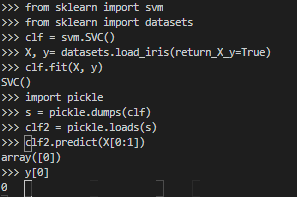
\includegraphics[width=10cm]{4.PNG}}
                \end{figure}
                \begin{itemize}
                    \item from sklearn import svm
                        \paragraph{}Mengimport svm dari library sklearn
                    \item from sklearn import datasets
                        \paragraph{}Mengimport datasets dari library sklearn
                    \item clf = svm.SVC()
                        \paragraph{}Membuat variable dengan nama clf dengan valuenya dari fungsi SVC dari file svm
                    \item X, y= datasets.load\_iris(return\_X\_y=True)
                    \item clf.fit(X, y)
                    \item import pickle
                    \item s = pickle.dumps(clf)
                    \item clf2 = pickle.loads(s)
                    \item clf2.predict(X[0:1])
                    \item y[0]
                \end{itemize}
            \item Conventions
                \begin{itemize}
                    \item Type Castign
                        \begin{figure}[ht]
                            \centerline{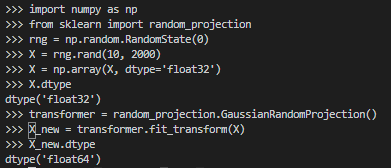
\includegraphics[width=10cm]{5.PNG}}
                        \end{figure}
                        \begin{itemize}
                            \item import numpy as np
                                \paragraph{}Mengimport numpy dengan menggunakan alias np
                            \item from sklearn import random\_projection
                                \paragraph{}Menimport random\_projection dari library sklearn
                            \item rng = np.random.RandomState(0)
                            \item X = rng.rand(10, 2000)
                            \item X = np.array(X, dtype='float32')
                            \item X.dtype
                            \item transformer = random\_projection.GaussianRandomProjection()
                            \item X\_new = transformer.fit\_transform(X)
                            \item X\_new.dtype
                        \end{itemize}
                    \item Refitting and updating parameters 
                        \begin{figure}[ht]
                            \centerline{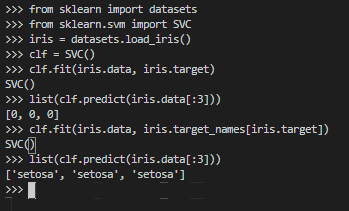
\includegraphics[width=10cm]{6.PNG}}
                        \end{figure}
                        \begin{itemize}
                            \item from sklearn import datasets
                                \paragraph{}Mengimport datasets dari library sklearn
                            \item from sklearn.svm import SVC
                                \paragraph{}Menimport fungsi SVC dari file svm dan library sklearn
                            \item iris = datasets.load\_iris()
                            \item clf = SVC()
                            \item clf.fit(iris.data, iris.target)
                            \item list(clf.predict(iris.data[:3]))
                            \item clf.fit(iris.data, iris.target\_names[iris.target])
                            \item list(clf.predict(iris.data[:3]))
                            \item 
                        \end{itemize}
                    \item Multiclass vs. multilabel fitting
                        \begin{figure}[ht]
                            \centerline{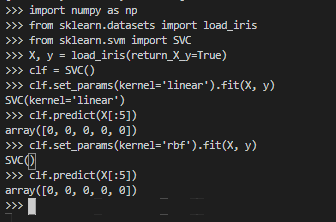
\includegraphics[width=10cm]{7.PNG}}
                        \end{figure}
                        \begin{itemize}
                            \item import numpy as np
                                \paragraph{}Menimport numpy dengan alian np
                            \item from sklearn.datasets import load\_iris
                                \paragraph{}Menimport load\_iris dari file datasets dan library sklearn
                            \item from sklearn.svm import SVC
                                \paragraph{}Menimport SVC dengan dari file svm pada library sklearn
                            \item X, y = load\_iris(return\_X\_y=True)
                            \item clf = SVC()
                            \item clf.se\_params(kernel='linear').fit(X, y)
                            \item clf.predict(X[:5])
                            \item clf.set\_params(kernel='rbf').fit(X, y)
                            \item clf.predict(X[:5])
                        \end{itemize}
                \end{itemize}
        \end{enumerate}
    \subsection{Error}
        \paragraph{}-

\end{document}


